\chapter{Soporte Simulado}
\label{chap:simulado}
Ahora que tenemos definidos cuales van a ser nuestros objetivos, y la infraestructura que vamos a utilizar para llevarlos acabo, en este capítulo, se va a hablar del proceso de integración en la plataforma de la parte simulada del robot. Pero antes de eso se darán unas nociones básicas de las características de este robot, para poder entender, el proceso de desarrollo. 
\section{Características del Lego Ev3}
\label{sec:caracteristicas}
Dentro de los robots de \textit{LEGO} el que mas versatilidad, además de más potencia de procesamiento y posibilidades en las opciones de creatividad a la hora de crear robots es \textit{LEGO MINDSTORMS Education}(Pack en el que viene integrado el \textit{LEGO Ev3}) tambien trae una mayor gama de sensores, por no decir que es uno de los lideres en la educación STEM (siglas en inglés de Ciencias, Tecnología,Ingeniería y Matemática), En el centro de \textit{LEGO MINDSTORMS Education} se encuentra el Bloque EV3, el bloque inteligente programable que controla motores y sensores y además proporciona comunicación inalámbrica como quiera que sea.
 \begin{figure}[H]
    \centering
    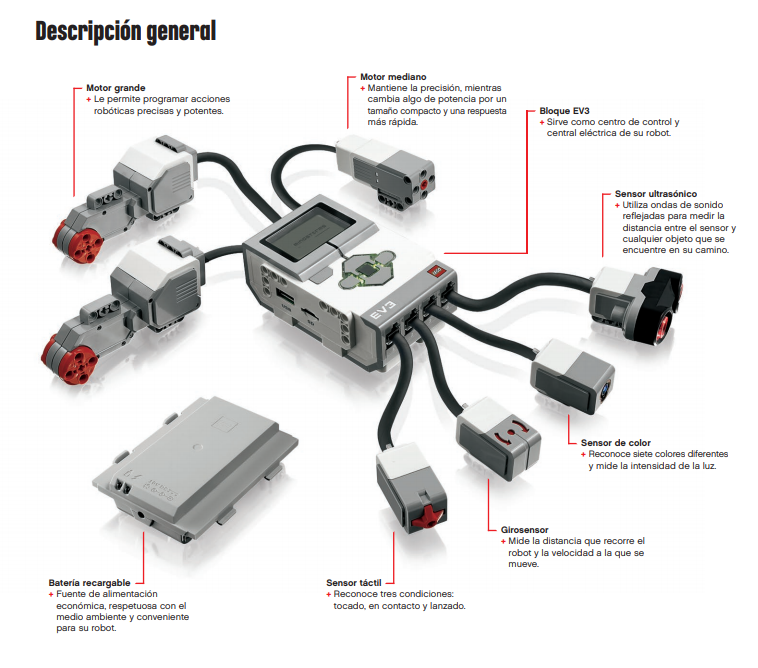
\includegraphics[scale=0.7]{img/partes.png}
    \caption{Conjunto Ev3} \label{fig:partes}
\end{figure}
 Esto quiere decir que las posibilidades a la hora de crear diferentes robots, con diferentes configuraciones de sensores, son prácticamente infinitas. Pero vamos a centrarnos en los casos que mas funcionalidad tienen. El robot que mas versatilidad presenta a la hora de superar ejercicios, es un robot triciclo, con dos ruedas delanteras y una pivotante trasera. Así que este será nuestro modelo para el robot. Y ademas como el \textit{kit de LEGO MINDSTORMS} viene con tres sensores diferentes, crearé tres modelos para integrarlos por separado en la plataforma.
  \begin{figure}[H]
    \centering
    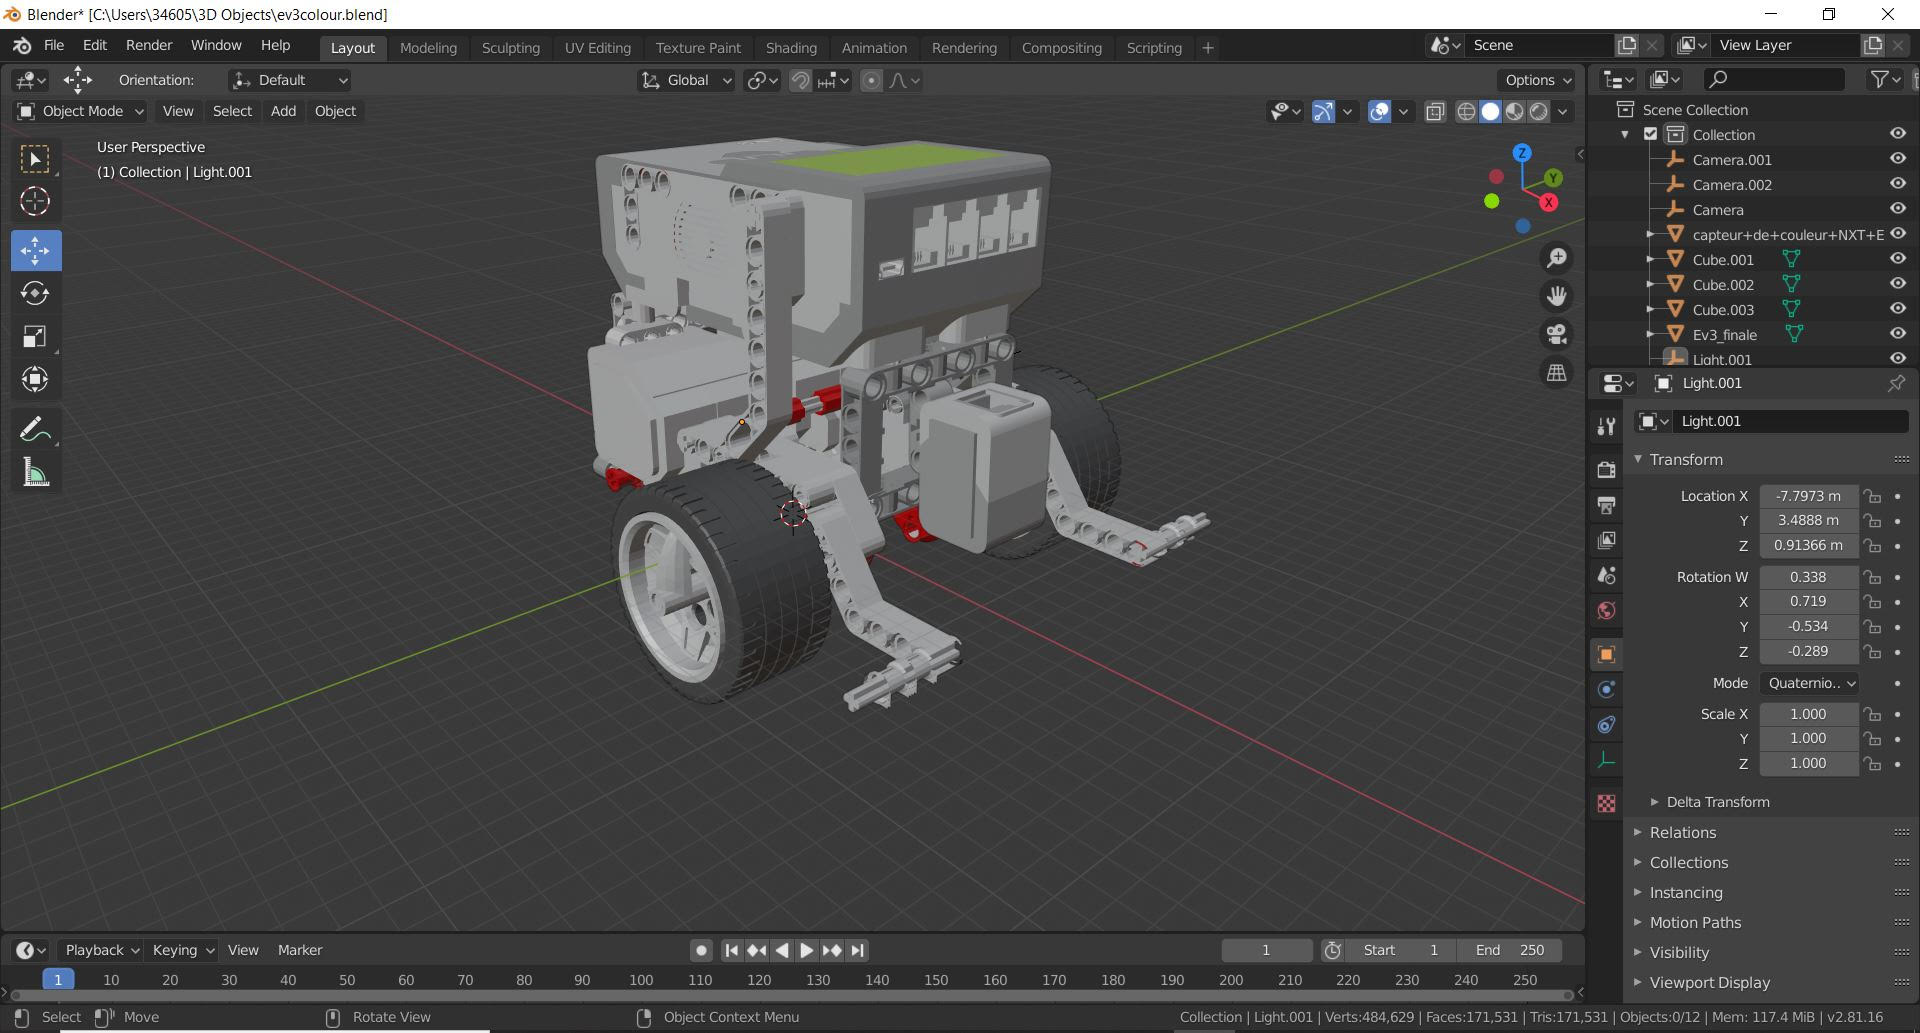
\includegraphics[width=0.7\textwidth]{img/blendercolor.jpg}
    \caption{Robot con sensor de color} \label{fig:color}
\end{figure}
 \begin{figure}[H]
    \centering
    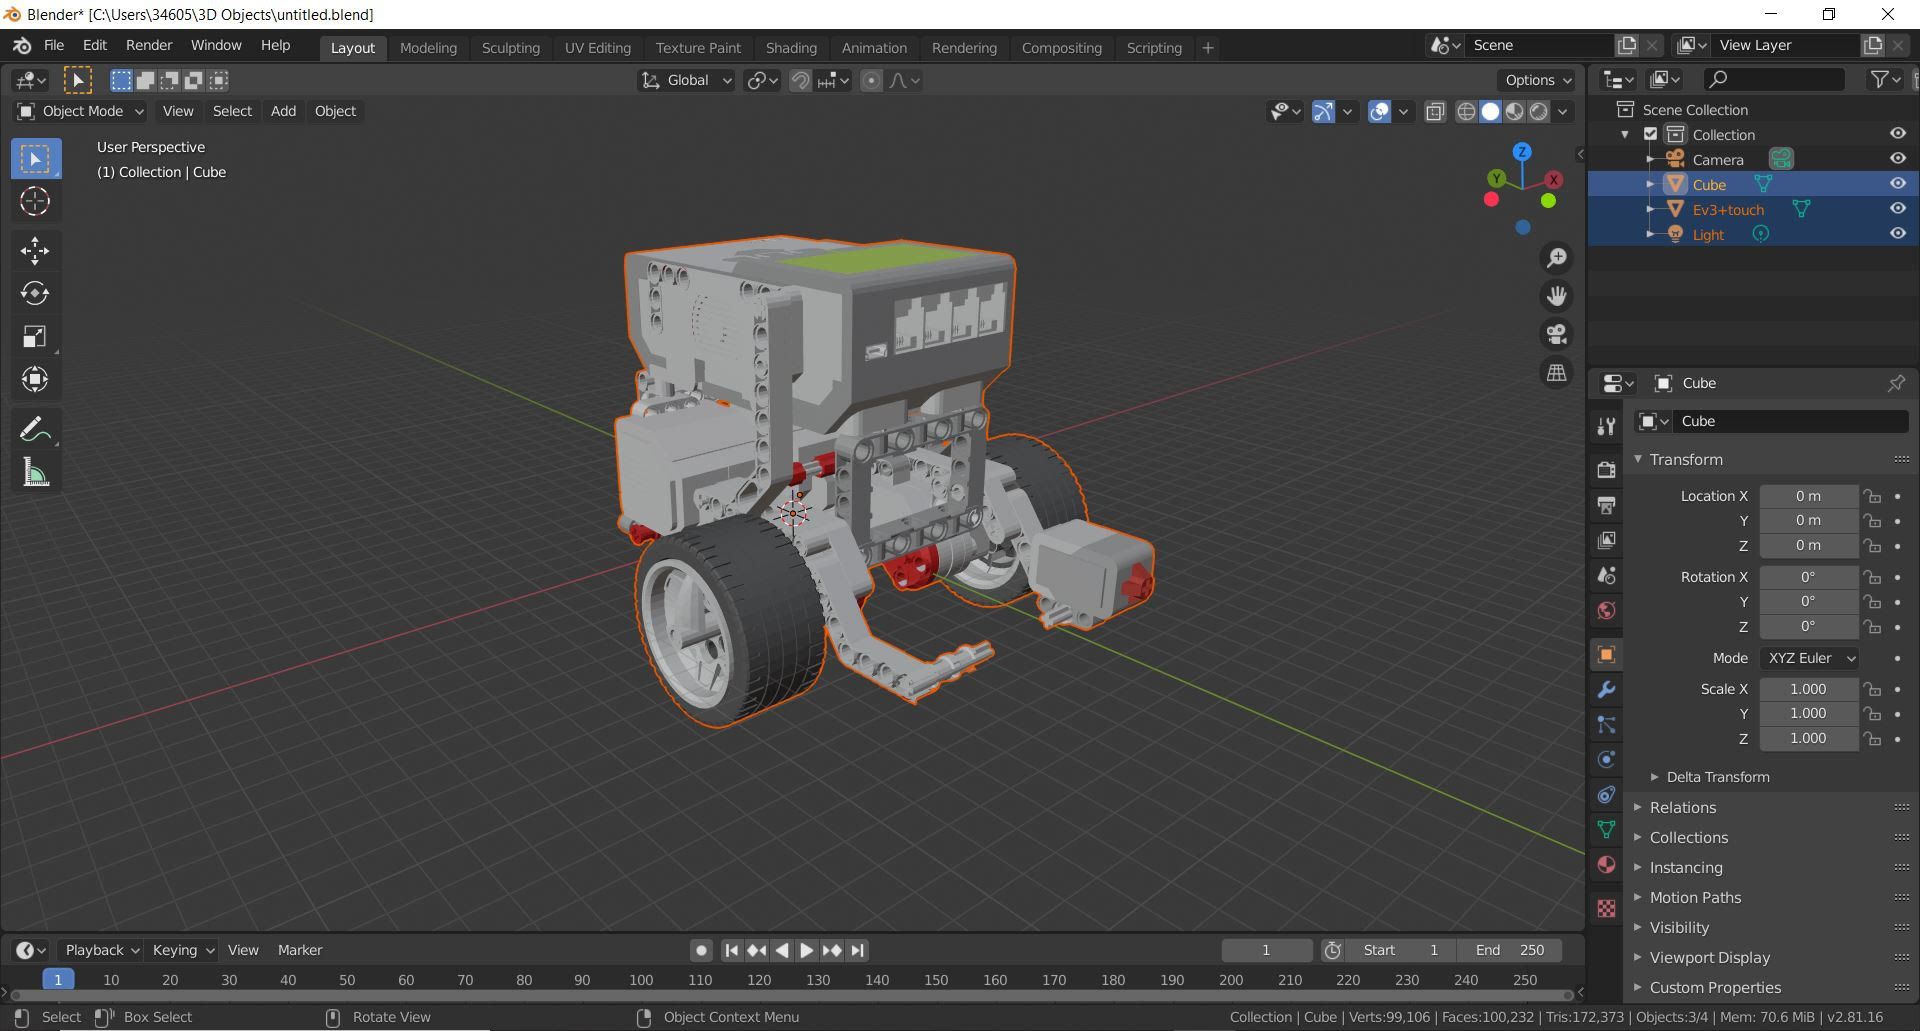
\includegraphics[width=0.7\textwidth]{img/blendertouch.jpg}
    \caption{Robot con sensor tactil} \label{fig:tactil}
\end{figure}
 \begin{figure}[H]
    \centering
    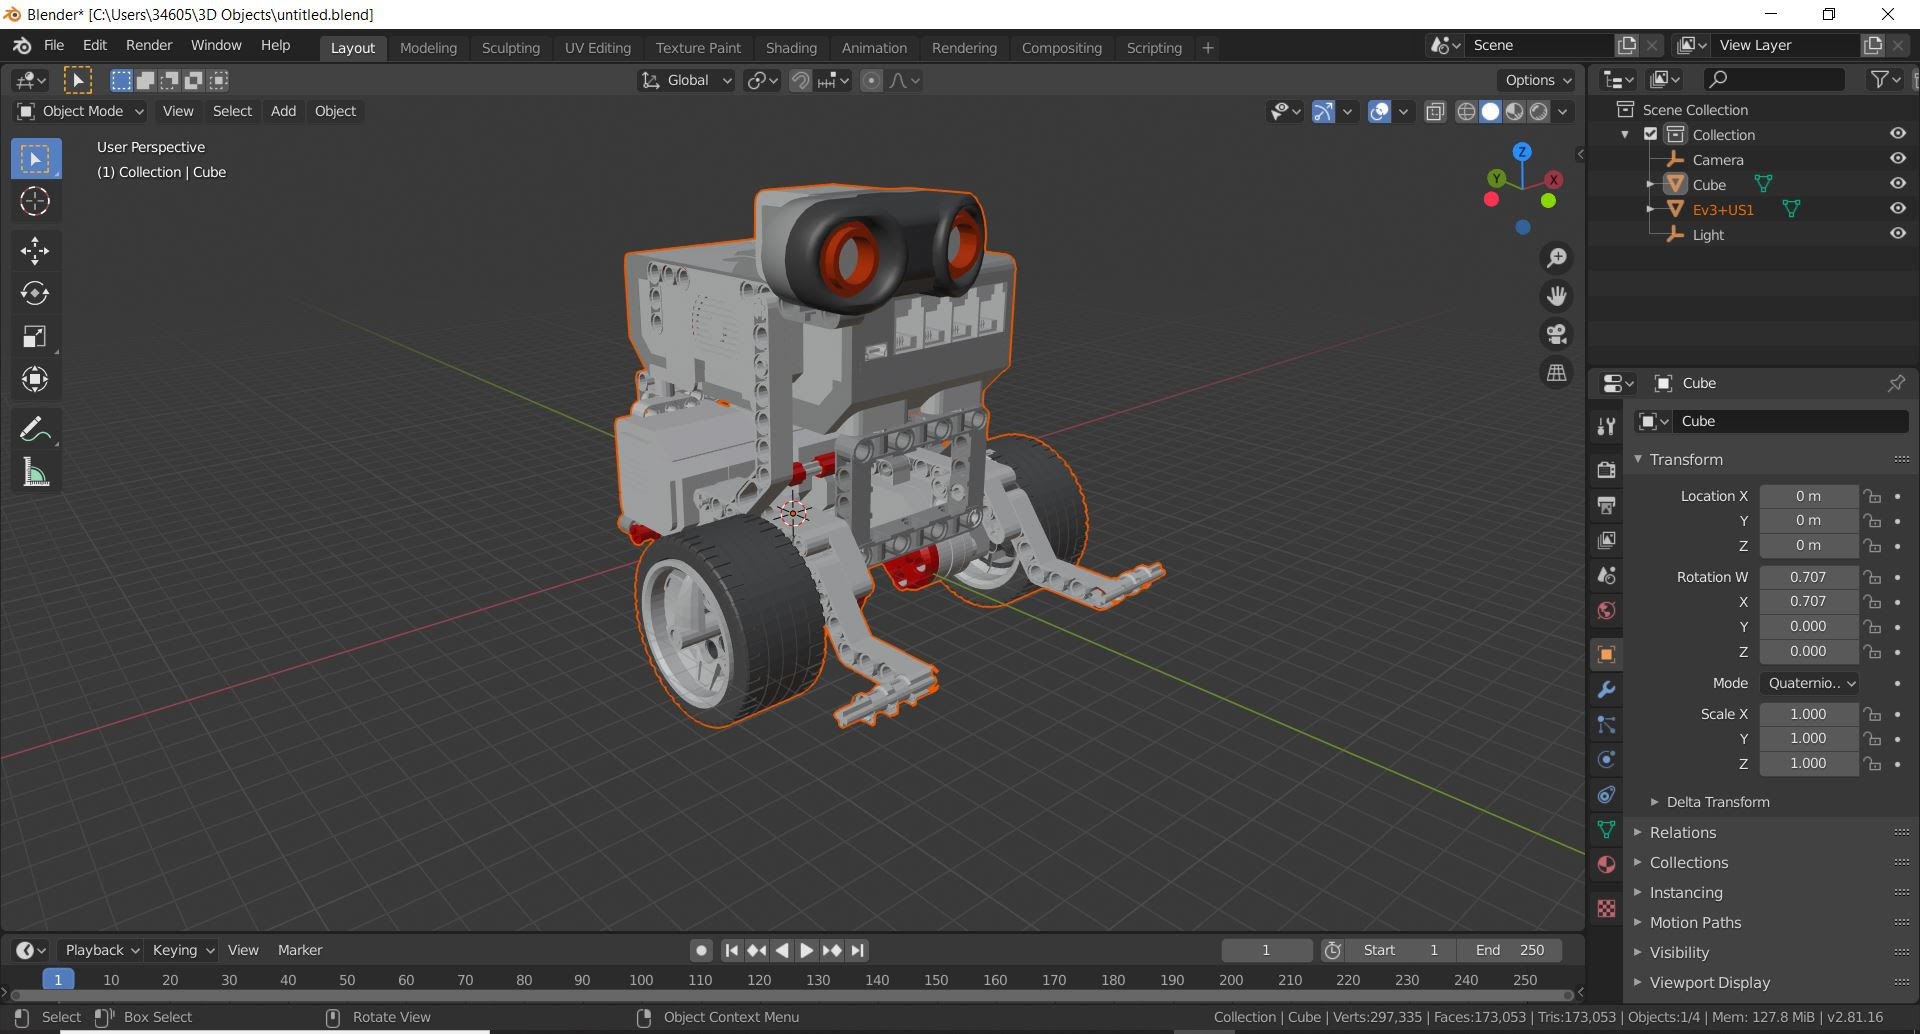
\includegraphics[width=0.7\textwidth]{img/blenderus.jpg}
    \caption{Robot con sensor de ultrasonidos} \label{fig:ultrasonidos}
\end{figure}
Para la tarea del modelaje 3D, he usado el programa de \textit{Blender}. \newline
Ahora que tenemos los tres modelos, voy a dividir el soporte del robot simulado en los diferentes sensores que implementar.
\section{Soporte de sensores}
\label{sec:sensores}

\subsection{Sensor de color}

El primer sensor que vamos a analizar es el sensor de color. El Sensor de color es un sensor digital que puede detectar el color o la intensidad de la luz que ingresa por la pequeña ventana de la cara del sensor. Este sensor puede utilizarse en tres modos diferentes: Modo color, Modo intensidad de la luz reflejada y Modo intensidad de la luz ambiental.\newline
La tasa de muestreo del sensor de color es de 1 kHz.
\begin{wrapfigure}{l}{0.3\linewidth}
    \centering
    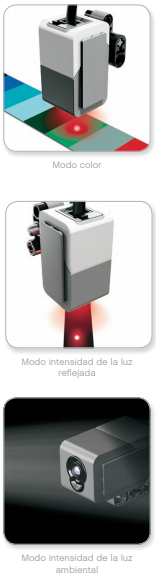
\includegraphics[width=0.6\linewidth]{img/color.png}
    \caption{Sensor color}{{\footnotesize Sensor de color en sus 3 usos}}
    \label{fig:color}
\end{wrapfigure}

\begin{itemize}
\item\textbf{En Modo color}, el Sensor de color reconoce siete colores: negro,
azul, verde, amarillo, rojo, blanco y marrón, además de Sin color.Esta capacidad de diferenciar los colores significa que su robot puede estar programado para clasificar pelotas o bloques de colores, y realizar acciones diferentes con cada color detectado.\newline
Este tipo de acciones, están ya contempladas en la funcionalidad del \textit{HAL API} de \textit{Kibotics}. Aunque en este caso utiliza una camara simulada para comprobar que color esta viendo.\newline
\textit{\textbf{getImage(cameraID)}}: Método que devuelve  \textit{robot}. 
    
    \begin{lstlisting}[language=javascript]
   function getImage(cameraID) {
    /**
     * Returns a screenshot from the robot camera
     */
    if (!cameraID || (this.camerasData.length === 1) || 
    (cameraID > this.camerasData.length - 1)) {
        return this.camerasData[0]['image'];
    } else {
        return this.camerasData[cameraID]['image'];
    }

}
    \end{lstlisting}
\end{itemize}

El \textit{LEGO EV3} no tiene una camara instalada, pero para el robot simulado, es lo mas sencillo de implementar, ya que puede analizar la imagen simulada y sacar el color RGB, para posteriormente dar nombre al color que ve.\newline
\textit{\textbf{getColorRGB()}}: Método que devuelve  \textit{RGB} en tres valores. 
    
    \begin{lstlisting}[language=javascript]
   function getObjectColorRGB(lowval, highval) {
    /**
     * This function filters an object in the scene with a given color, uses OpenCVjs to filter
     * by color and calculates the center of the object.
     *
     * Returns center: CenterX (cx), CenterY (cy) and the area of the object detected in the image.
     */

    if (lowval.length === 3) {
        lowval.push(0);
    }
    if (highval.length === 3) {
        highval.push(255);
    }
    var image = this.getImage();
    var binImg = new cv.Mat();
    var M = cv.Mat.ones(5, 5, cv.CV_8U);
    var anchor = new cv.Point(-1, -1);
    var lowThresh = new cv.Mat(image.rows, image.cols, image.type(), lowval);
    var highThresh = new cv.Mat(image.rows, image.cols, image.type(), highval);
    var contours = new cv.MatVector();
    var hierarchy = new cv.Mat();

    cv.morphologyEx(image, image, cv.MORPH_OPEN, M, anchor, 2,
        cv.BORDER_CONSTANT, cv.morphologyDefaultBorderValue()); // Erosion followed by dilation

    cv.inRange(image, lowThresh, highThresh, binImg);
    cv.findContours(binImg, contours, hierarchy, cv.RETR_CCOMP, cv.CHAIN_APPROX_SIMPLE);
    if (contours.size() > 0) {

        let stored = contours.get(0);
        var objArea = cv.contourArea(stored, false);

        let moments = cv.moments(stored, false);
        var cx = moments.m10 / moments.m00;
        var cy = moments.m01 / moments.m00;

    }
    return {center: [parseInt(cx), parseInt(cy)], area: parseInt(objArea)};
}
    \end{lstlisting}
    
Una vez realizado este paso podemos ponerle un nombre al color, como hace el \textit{LEGO EV3} real.

\begin{itemize}
\item\textbf{En Modo intensidad de la luz reflejada}, el Sensor de color mide la intensidad de la luz que se refleja desde una lámpara emisora de luz color rojo. El sensor utiliza una escala de 0 (muy oscuro) a 100 (muy luminoso). Esto significa que su robot puede estar programado para moverse sobre una superficie blanca hasta detectar una línea negra o para interpretar una tarjeta de identificación con código de color.
Esto en el robot simulado, es diferente, ya que no podemos ver como una magnitud física como es la luz se refleja un objeto, pero este efecto depende del color que se este viendo en la imagen, la luminosidad del color se puede calcular con esta función:

\textit{\textbf{getLightness(valuemin, valuemax)}}: Método que devuelve  \textit{Luminosidad}. 
    
    \begin{lstlisting}[language=javascript]
   function getLightness(valuemin, valuemax) {
    
    let image = this.getObjectColorRGB(valuemin, valuemax);
    let L = ((image.center[0]- image.center[1])/2)*100/255;
    
    /**
     * Returns lightness with a percent
     */
    
    return L.

}
\end{lstlisting}

Esta funcion puede resultar util, para, por ejemplo, poder seguir una linea, cuando haya colores muy similares, o cuando se este utilizando el robot en una mesa o superficie alta, detectar antes, donde esta el borde.

\item\textbf{En Modo intensidad de la luz ambiental}, el Sensor de color mide la intensidad de la luz que ingresa en la ventana desde su entorno, como la luz del sol o el haz de una linterna. El sensor utiliza una escala de 0 (muy oscuro) a 100 (muy luminoso). Esta funcionalidad, no puede ser implementada en la plataforma, ya que no tenemos un foco de luz que se puede analizar, ni tampoco una magnitud dentro del entorno que represente la luz.

\end{itemize}

\subsection{Sensor de ultrasonido}

El Sensor ultrasónico es un sensor digital que puede medir la
distancia a un objeto que se encuentra frente a él. Para hacerlo,
envía ondas de sonido de alta frecuencia y mide cuánto tarda el
sonido en reflejarse de vuelta al sensor. La frecuencia de sonido
es demasiado alta para el oído humano.
La distancia a un objeto puede medirse en pulgadas o centímetros.
Esto le permite programar su robot para que se detenga a una
distancia determinada de una pared.
Al utilizar unidades en centímetros, la distancia detectable es entre
3 y 250 centímetros (con una exactitud de +/- 1 centímetro). Al utilizar
unidades en pulgadas, la distancia detectable es entre 1 y 99
pulgadas (con una exactitud de +/- 0,394 pulgadas). Un valor de
255 centímetros o 100 pulgadas significa que el sensor no puede
detectar ningún objeto frente a él.\newline
\begin{wrapfigure}{r}{0.5\linewidth}
    \centering
    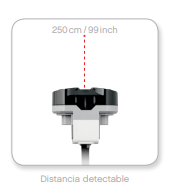
\includegraphics[width=0.5\linewidth]{img/ultrasonidos.png}
    \caption{Sensor de ultrasonidos}
    \label{fig:ultrasonido}
\end{wrapfigure}
En \textit{Kibotics} la implementación que hay para las distancias es  usar un \textit{RayCaster}. Que es equivalente a poner láseres apuntando hacia todas direcciones por delante del robot de estaa forma:


\textit{\textbf{Funciones que calculan la distancia}}: Método que devuelve  un unico valor con la distancia mas corta. 

 \begin{lstlisting}[language=javascript]
function getDistance() {
    /**
     * This function returns the distance for the raycaster in the center of the arc of rays.
     */
    var distances = this.getDistances();

    if (distances[13] !== 10 || distances[14] !== 10 || distances[15] !== 10 || distances[16] !== 10 || distances[17] !== 10) {
        let distance0 = 100;
        let distance1 = 100;
        let distance2 = 100;
        let distance3 = 100;
        let distance4 = 100;
        if (distances[13] !== 10) {
            distance0 = distances[13];
        }
        if (distances[14] !== 10) {
            distance1 = distances[14];
        }
        if (distances[15] !== 10) {
            distance2 = distances[15];
        }
        if (distances[16] !== 10) {
            distance3 = distances[16];
        }
        if (distances[17] !== 10) {
            distance4 = distances[17];
        }
        let min_distances = [distance0, distance1, distance2, distance3, distance4];
        Array.min = function (array) {
            return Math.min.apply(Math, array);
        };
        return Array.min(min_distances);
    } else {
        return 10;
    }
}

function getDistances() {
    /**
     * This function returns an array with all the distances detected by the rays.
     */
    var distances = [];
    for (var i = 0; i <= 31; i++) {
        distances.push(10);
    }
    var groups = ["center", "right", "left"];
    for (i = 0; i < groups.length; i++) {
        this.distanceArray[groups[i]].forEach((obj) => {
            if (typeof obj.d != "undefined") {
                distances[obj.id] = obj.d;
            }
        });
    }
    return distances;
}
\end{lstlisting}


\section{Nuevos ejercicios individuales}
\label{sec:escenarios}

Se han incorporado nuevos escenarios a \textit{WebSim} que dan la posibilidad de realizar nuevos ejercicios y mejorar los ya disponibles. En esta sección se explicarán los nuevos ejercicios desarrollados con un solo \textit{robot} en escena y sus soluciones en \textit{Scratch}.

\subsection{Sigue-líneas visión}
    Este ejercicio consiste en seguir una línea blanca en el suelo sobre fondo negro haciendo uso de la cámara del \textit{robot}, que recoge las imágenes y las filtra para poder seguirla.
    
    Se ha mejorado el escenario cambiando la textura del suelo a una creada con la trazada del circuito de Interlagos de Fórmula 1. Se ha realizado con un programa de diseño gráfico (\textit{Photoshop}) y, debido a su peso computacional, se ha reducido posteriormente su tamaño para aliviar los tiempos de carga. 
    
    \begin{figure}[H]
    \centering
    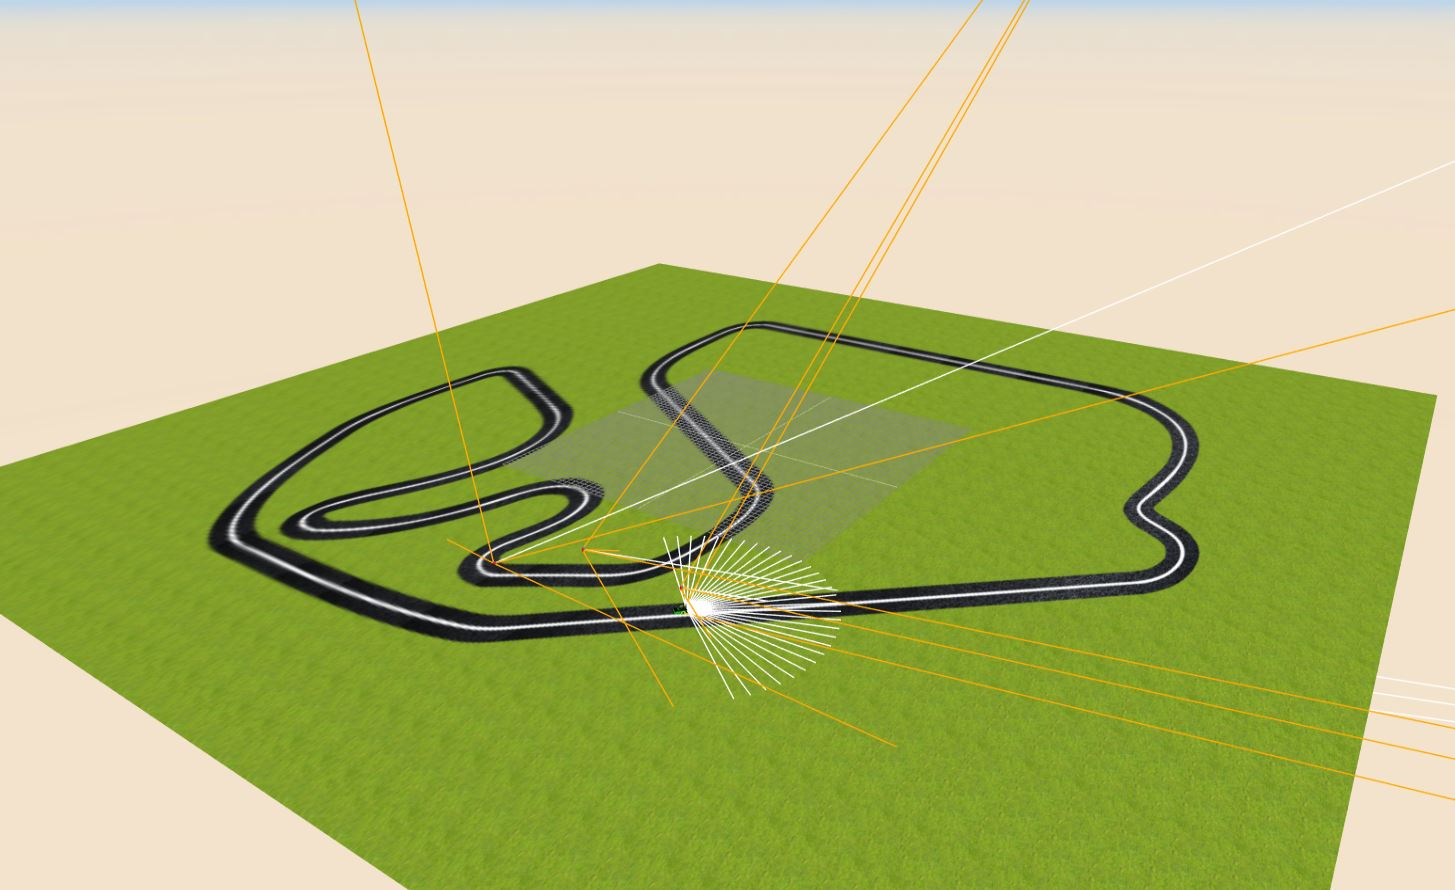
\includegraphics[scale=0.4]{img/pibot_vision.JPG}
    \caption{Escenario para el ejercicio \textit{piBot} sigue-líneas con cámara} \label{fig:siguelineavision}
    \end{figure}
    
        \begin{figure}[H]
    \centering
    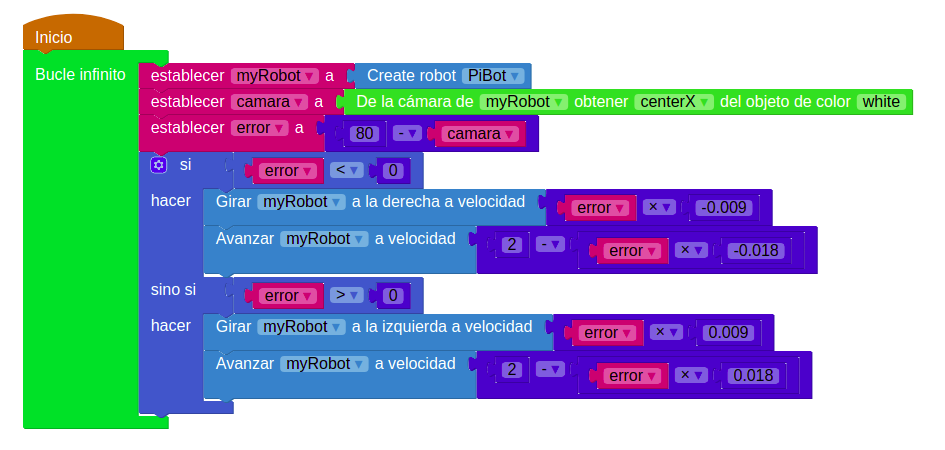
\includegraphics[scale=0.5]{img/siguelineasvisioncodigo.png}
    \caption{Solución en \textit{Scratch} para el ejercicio sigue-líneas visión} 
    \label{fig:visionSolution}
    \end{figure}
    
    En esta solución\footnote{\url{https://youtu.be/fRq__W_BETk}} se comanda velocidad lineal al robot y utiliza el bloque que obtiene el centro del eje X de los objetos blancos. Según el valor obtenido, se gira el \textit{robot} en un sentido u otro.
    
\subsection{Sigue-líneas infrarrojos}
     Este ejercicio consiste en seguir una línea negra en el suelo sobre fondo blanco haciendo uso de los sensores infrarrojos del \textit{robot} que apuntan hacia abajo. 
     
    Tiene un recorrido similar a sigue-líneas visión, pero con fondo blanco y recorrido negro para facilitar la implementación de código en el robot real y que no haya que realizar modificaciones. Para que funcionara correctamente ha sido necesario añadir el color blanco a \textit{undestandedColors} para realizar el filtro y poder pasar ``\textit{white}'' como atributo a la función \textit{getObjectColor()}.
    
    \begin{figure}[H]
    \centering
    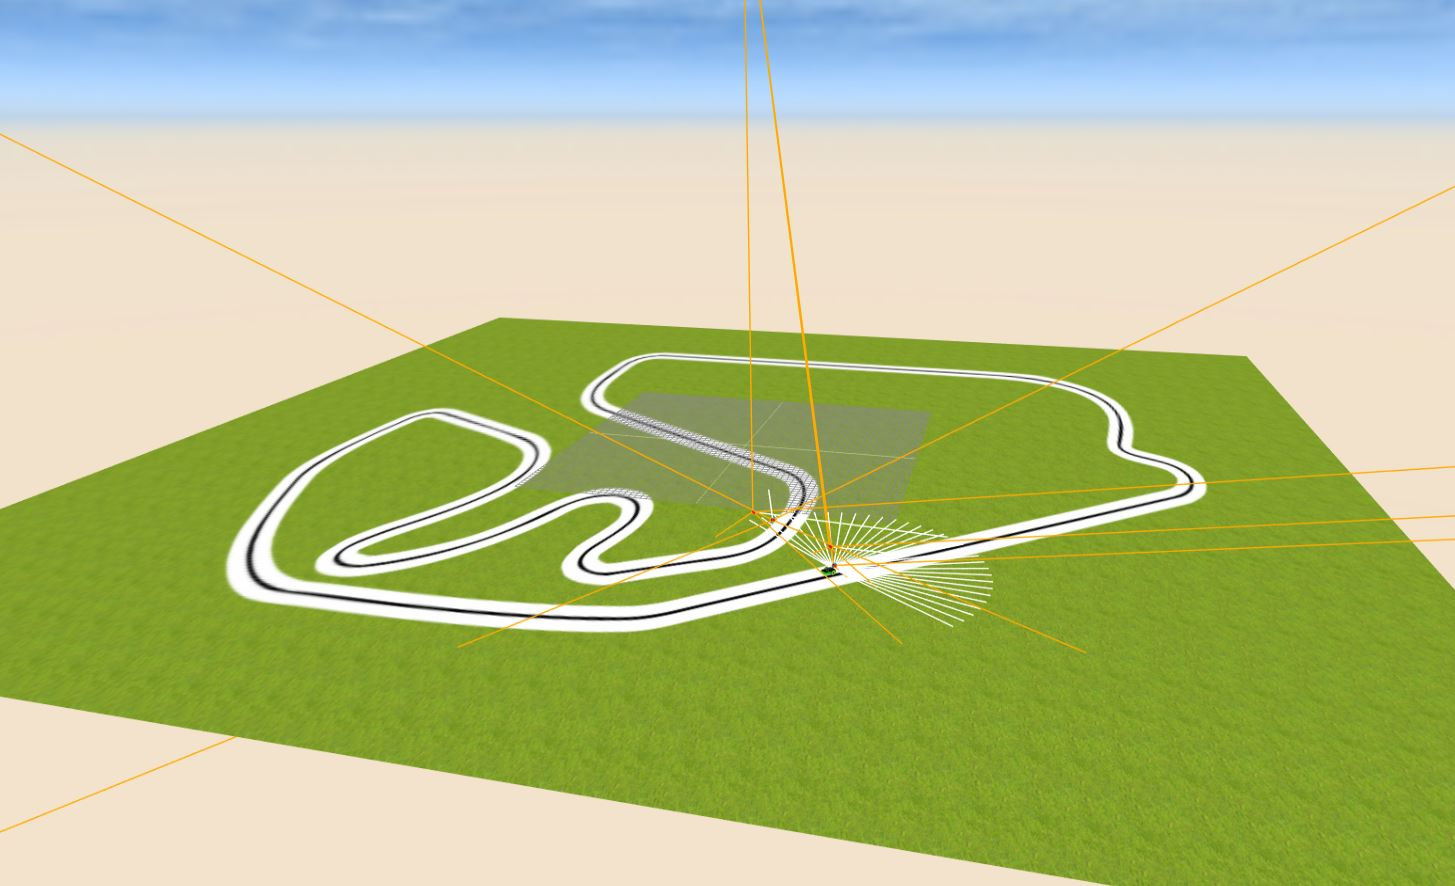
\includegraphics[scale=0.3]{img/siguelineas_ir.JPG}
    \caption{Escenario para el ejercicio para el \textit{robot piBot} sigue-líneas infrarrojos} \label{fig:siguelineasIR}
    \end{figure}
    
           \begin{figure}[H]
    \centering
    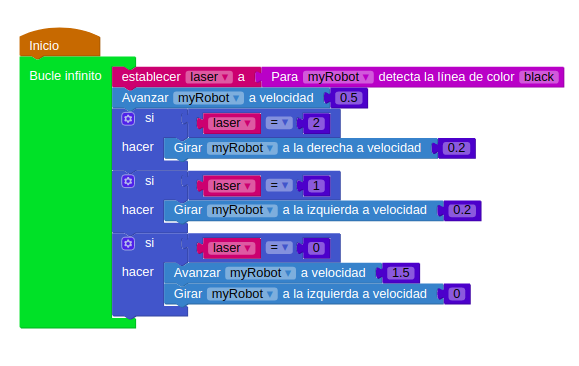
\includegraphics[scale=0.6]{img/siguelineaIRcodigo.png}
    \caption{Solución en \textit{Scratch} para el ejercicio sigue-líneas infrarrojos} 
    \label{fig:irSolution}
    \end{figure}
    
    En esta solución\footnote{\url{https://youtu.be/d4HETtPmahA}} se comanda una velocidad lineal y se obtienen los valores de los sensores infrarrojos del \textit{robot} y se comanda una velocidad angular en función de dónde detecte la línea.
    
\subsection{Choca-gira}
\label{subsec:chocagira}
En este ejercicio hay programar al \textit{robot} para que avance recto mientras no haya obstáculos haciendo uso del sensor de ultra-sonidos. Si encuentra un obstáculo, tiene que detenerse, retroceder un poco, girar un ángulo aleatorio y reemprender la marcha.

Escenario creado en \textit{Blender} con un aspecto similar a su análogo en el simulador \textit{Gazebo}. Para ello se han adaptado la mayor parte de las estructuras que dispone el escenario original para su integración en \textit{WebSim}. 

    \begin{figure}[H]
    \centering
    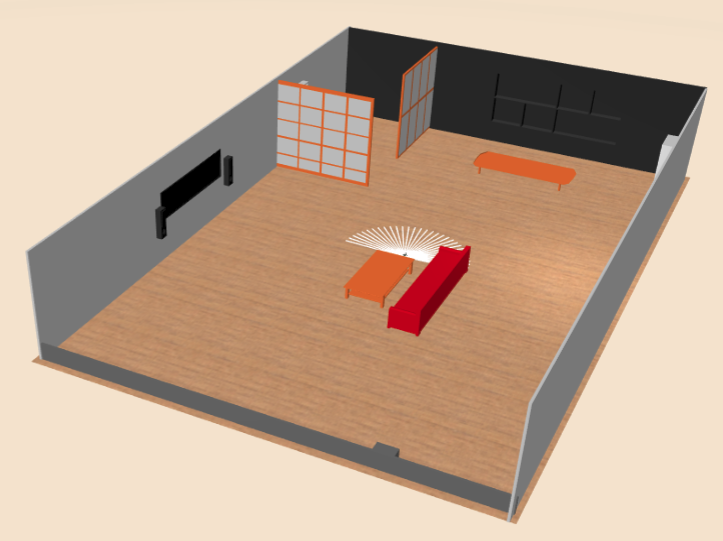
\includegraphics[scale=0.5]{img/bump&go.png}
    \caption{Escenario para el ejercicio choca-gira} \label{fig:chocagira}
    \end{figure}
    \begin{figure}[H]
    \centering
    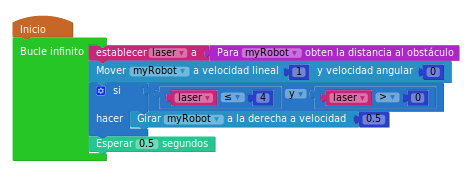
\includegraphics[scale=0.75]{img/chocagiracodigo.png}
    \caption{Solución en \textit{Scratch} para el ejercicio choca-gira} 
    \label{fig:chocagiraSolution}
    \end{figure}
    En esta solución\footnote{\url{https://youtu.be/lXL3lTbgp_E}} se obtienen los valores del sensor de ultra-sonidos y se comanda una velocidad lineal. Si encuentra un obstáculo se gira a la derecha durante 0.5 segundos.
    
\subsection{Sigue-pelota}
\label{subsec:pelota}

Este ejercicio consiste en seguir una pelota en movimiento. Hay que emplear las imágenes obtenidas por el \textit{robot} y programar la lógica de control que permita seguir la pelota.

Se ha realizado dos escenarios distintos, uno para \textit{PiBot} y otro para \textit{drone}.
Ambos disponen de una pelota de color negro, que debe ser seguida usando la cámara del \textit{robot}, a la que se le ha dado movimiento a través de primitivas de \textit{A-Frame}. En la figura \ref{fig:secuenciaDrone} se puede ver una secuencia con la animación de una pelota y en el siguiente código se muestra el archivo de configuración de este ejercicio, que incluye esa animación de \textit{A-Frame}:\\

\begin{lstlisting}[language=json]
{
  "robot": {
    "model":"../assets/models/drone_animation.gltf",
    "scale": "0.5 0.5 0.5",
    "position":"12 1 25",
    "rotation": "0 50 0"
  },
  "gravity": 0,
  "ground": "../assets/textures/escenarioLiso.png",
  "sky": "../assets/textures/sky.png",
  "secondaryCamera": "4 20 30",
  "cameraRobot":"0 0.03 -0.01",
  "objects":[
        {
      "type": "a-sphere",
      "id":"redBall",
      "position": "4 15 20",
      "color": "#000000",
      "radius": "1.5",
      "animation":"property: position; from: 4 15 20 ;to: 0 15 -20; dir: alternate; dur: 10000; loop: true",
      "animation__2":"property: position; from: 0 15 -20 ;to: 0 2 -20 ; delay: 10000; dir: alternate; dur: 10000; loop: true",
      "animation__3":"property: position; from: 0 2 -20 ;to: 4 2 20 ; delay: 20000; dir: alternate; dur: 10000; loop: true",
      "animation__4":"property: position; from: 4 2 20 ;to: 4 15 20; delay: 30000; dir: alternate; dur: 10000; loop: true",
      "animation__5":"property: position; from: 4 15 20 ;to: -10 15 10; delay: 40000; dir: alternate; dur: 10000; loop: true",
      "animation__6":"property: position; from: -10 15 10 ;to: 20 8 -30; delay: 50000; dir: alternate; dur: 10000; loop: true"
      }
      ]
}
\end{lstlisting} 


 Haciendo especial mención al campo \textit{objects}, en el que se crea una pelota negra con la animación indicada en todos los campos \textit{animation} y genera el siguiente elemento en \textit{HTML}, que incluye en el \textit{DOM}:

\begin{lstlisting}[language=html]
<a-sphere id="blackBall" position="12 1 25" color="#000000" radius="1.5" 
    animation="property: position; from: 4 15 20 ;to: 0 15 -20; dir: alternate; dur: 10000; loop: true"
    animation__2="property: position; from: 0 15 -20 ;to: 0 2 -20 ; delay: 10000; dir: alternate; dur: 10000; loop: true" 
    animation__3="property: position; from: 0 2 -20 ;to: 4 2 20 ; delay: 20000; dir: alternate; dur: 10000; loop: true" 
    animation__4="property: position; from: 4 2 20 ;to: 4 15 20; delay: 30000; dir: alternate; dur: 10000; loop: true" 
    animation__5= "property: position; from: 4 15 20 ;to: -10 15 10; delay: 40000; dir: alternate; dur: 10000; loop: true" 
    animation__6="property: position; from: -10 15 10 ;to: 20 8 -30; delay: 50000; dir: alternate; dur: 10000; loop: true">
</a-sphere>
\end{lstlisting}


\begin{figure}[H]
\begin{subfigure}[t]{0.3\textwidth}
  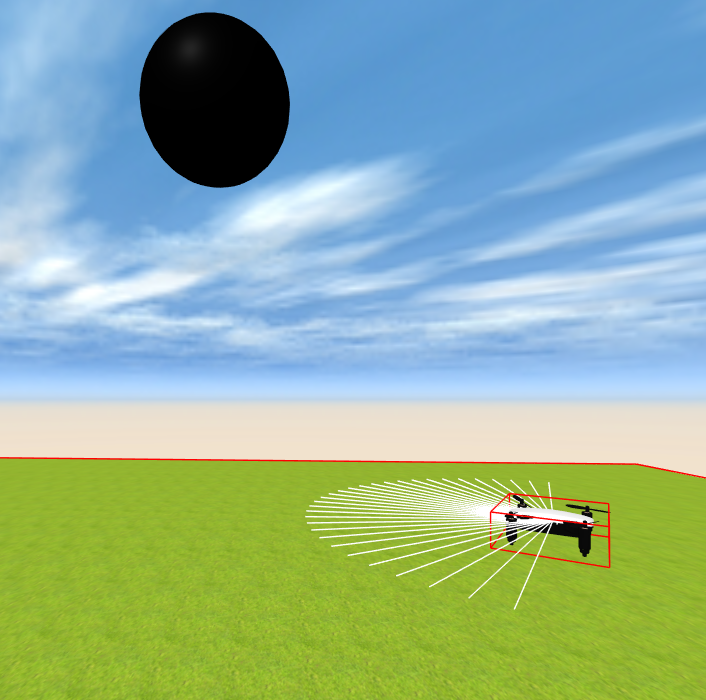
\includegraphics[width=4cm, height=4cm]{img/followBallTello12.png}
\label{fig:figure2_2}
\end{subfigure}\hfill
\begin{subfigure}[t]{0.3\textwidth}
    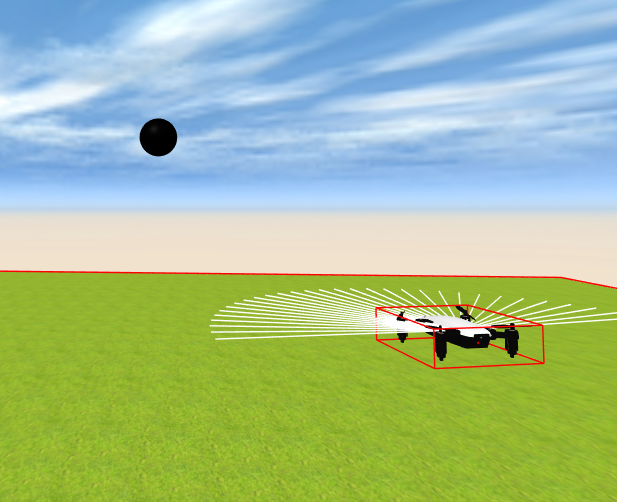
\includegraphics[width=4cm, height=4cm]{img/followBallTello22.png}
\label{fig:figure2_3}
\end{subfigure}\hfill
\begin{subfigure}[t]{0.3\textwidth}
    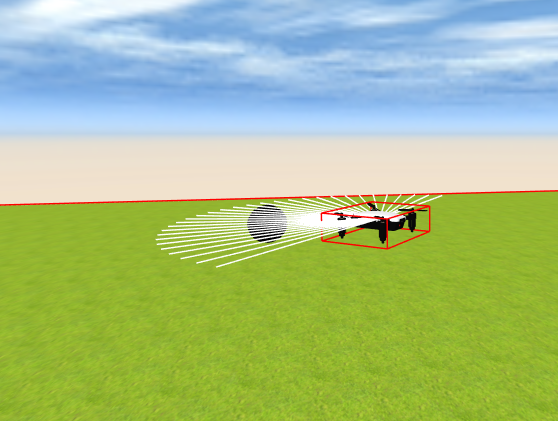
\includegraphics[width=4cm, height=4cm]{img/followBallTello32.png}
\label{fig:figure2_4}
\end{subfigure}
\begin{subfigure}[t]{0.3\textwidth}
    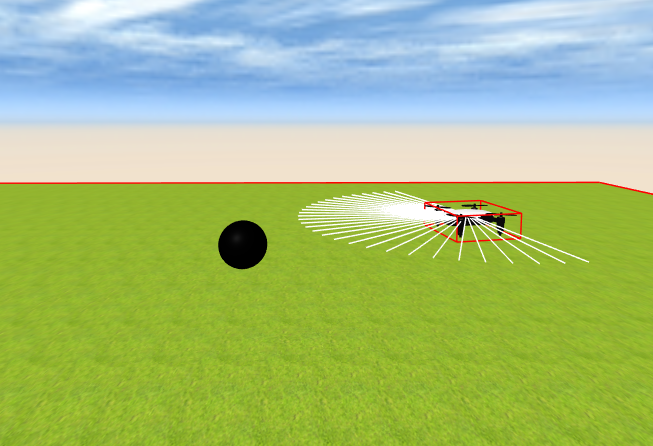
\includegraphics[width=4cm, height=4cm]{img/followBallTello42.png}
\label{fig:figure2_6}
\end{subfigure}\hfill
\begin{subfigure}[t]{0.3\textwidth}
    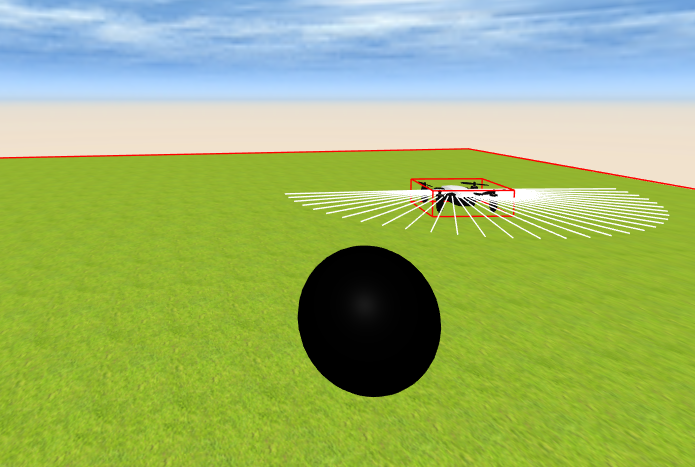
\includegraphics[width=4cm, height=4cm]{img/followBallTello52.png}
\label{fig:figure2_7}
\end{subfigure}\hfill
\begin{subfigure}[t]{0.3\textwidth}
    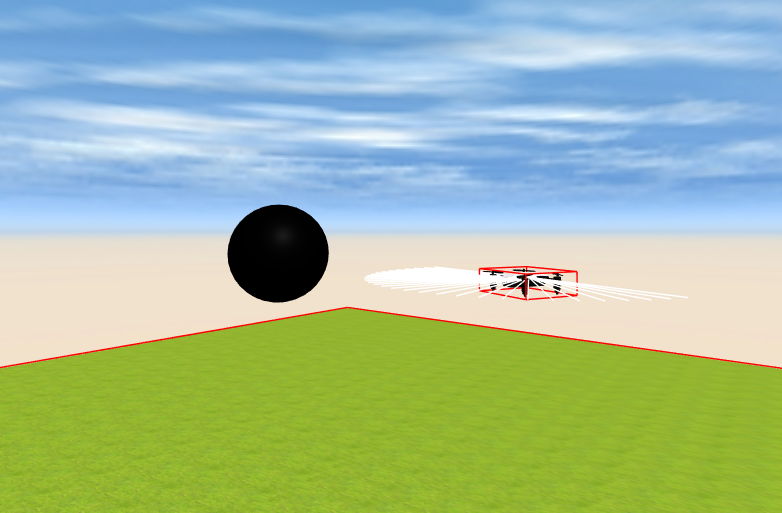
\includegraphics[width=4cm, height=4cm]{img/followBallTello62.png}
\label{fig:figure2_8}
\end{subfigure}

\caption{Secuencia del ejercicio \textit{drone} sigue-pelota}
\label{fig:secuenciaDrone}
\end{figure}


    \begin{figure}[h]
    \centering
    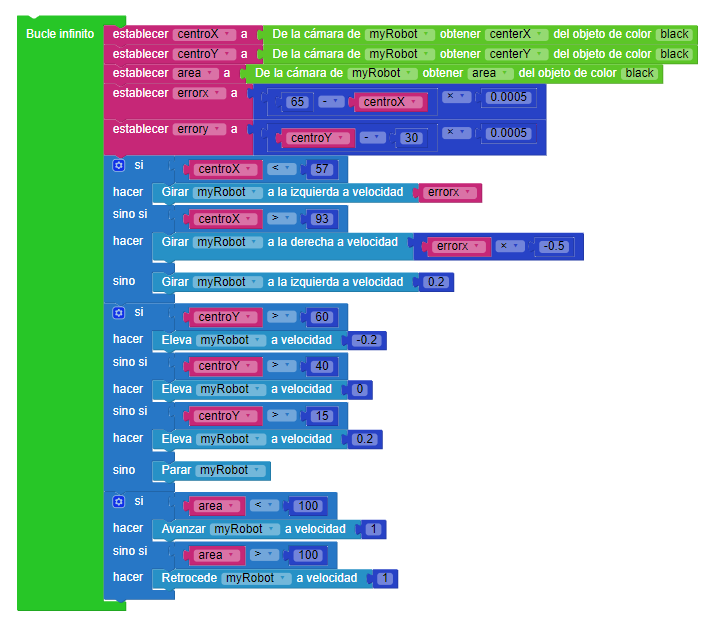
\includegraphics[scale=0.9]{img/siguepelotacodigo.png}
    \caption{Solución en \textit{Scratch} para el ejercicio sigue pelota drone} 
    \label{fig:pelotaSolution}
    \end{figure}
    La solución de este ejercicio\footnote{\url{https://youtu.be/XQrNaWxRg7U}} se ha realizado obteniendo toda la información que aporta la cámara, tanto la posición del objeto en el eje X e Y de la imagen como su área. Según los valores obtenidos se comandan distintas velocidades angulares y lineales. 
\subsection{Atraviesa-bosque}
\label{subsec:atraviesabosque}
Ejercicio basado en atravesar un pasillo con diversos objetos que hay que esquivar. El sensor necesario es el infrarrojos para detectar en que posición se encuentra cada uno de los obstáculos. El escenario y los obstáculos se han creado con primitivas de \textit{A-Frame}.

    \begin{figure}[H]
    \centering
    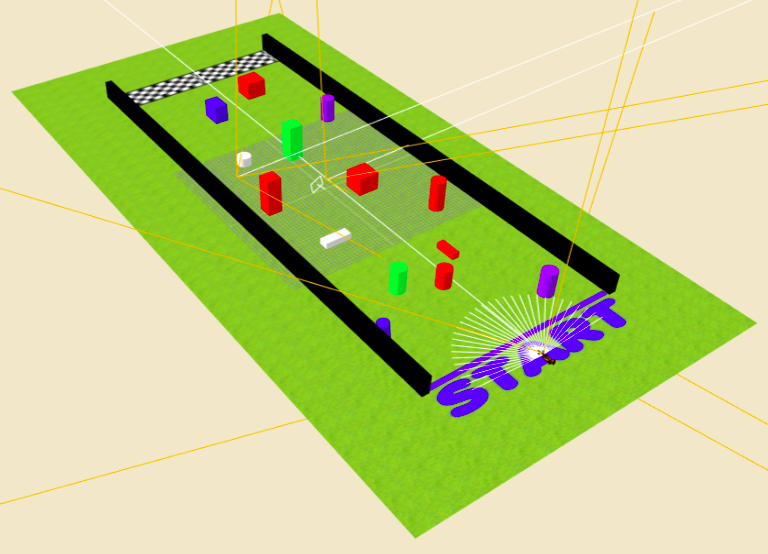
\includegraphics[scale=0.45]{img/atraviesabosque-indiv.png}
    \caption{Escenario para el ejercicio atraviesa bosque} 
    \label{fig:atraviesaBosqueind}
    \end{figure}

    \begin{figure}[H]
    \centering
    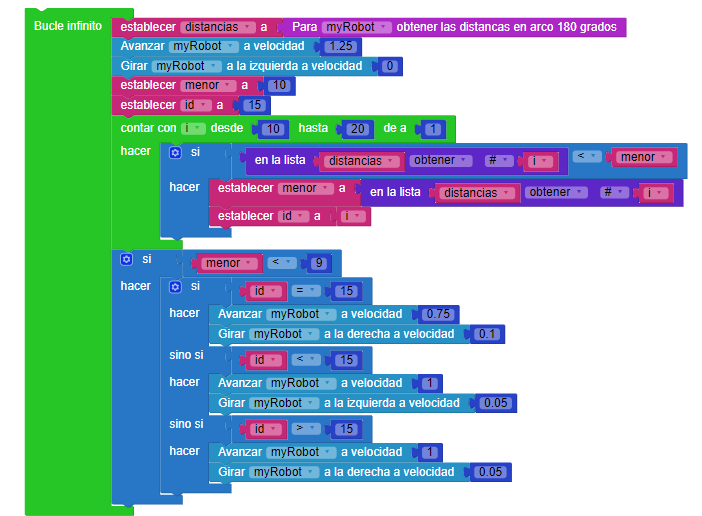
\includegraphics[scale=0.6]{img/atraviesaBosqueCodigo.png}
    \caption{Solución en \textit{Scratch} para el ejercicio atraviesa bosque} 
    \label{fig:bosqueSolution}
    \end{figure}
    
    En esta solución\footnote{\url{https://youtu.be/z3n47wWHDFc}} se obtienen todos los valores que devuelve el sensor de ultra-sonidos y, según donde detecte el obstáculo, gira en un sentido u otro.

\subsection{Cuadrado con drone}
Este ejercicio consiste en comandar velocidades al \textit{drone} para dibujar un cuadrado con el movimiento del \textit{robot}.

    \begin{figure}[H]
        \centering
        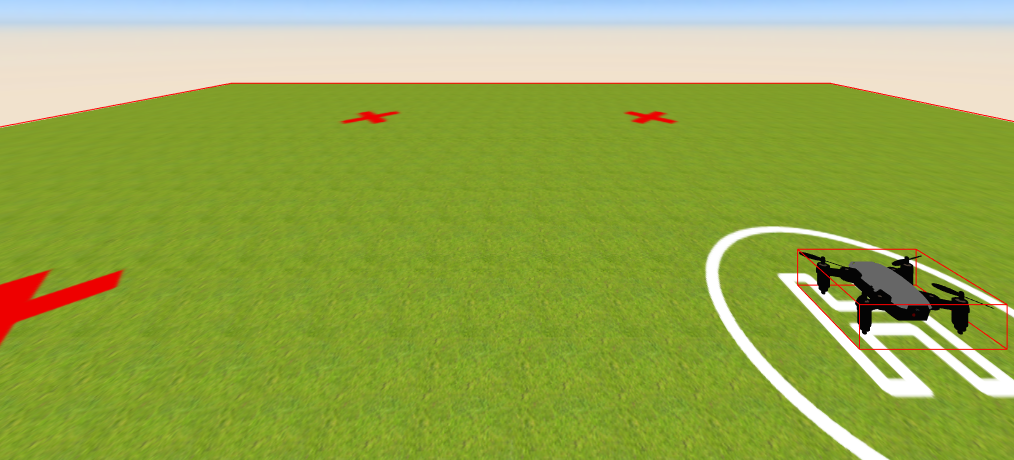
\includegraphics[scale=0.4]{img/cuadradoDrone.png}
        \caption{Escenario de WebSim para el ejercicio drone cuadrado} 
        \label{fig:droneCuadrado}
    \end{figure}

    \begin{figure}[H]
    \centering
    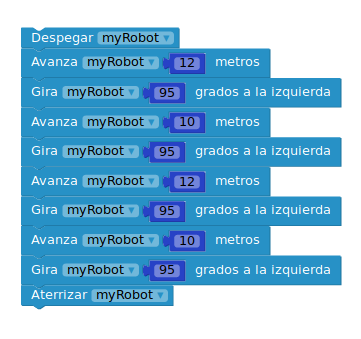
\includegraphics[scale=0.5]{img/tellocuadradocodigo.png}
    \caption{Solución en \textit{Scratch} para el ejercicio cuadrado drone} 
    \label{fig:cuadradoSolution}
    \end{figure}
    Su solución\footnote{\url{https://www.youtube.com/watch?v=XjQNhNCkOJA}} consiste en avanzar los metros necesarios para llegar a la cruz y, cuando se ha completado el desplazamiento, girar 90 grados aproximadamente para así ``dibujar'' un cuadrado repitiendo este proceso.
    
\section{Ejercicios competitivos}
\label{sec:competitive}
Uno de los objetivos de este proyecto era añadir ejercicios competitivos a \textit{Kibotics} sobre el simulador \textit{WebSim}. Se hace especial mención a ellos debido a que son completamente diferentes al resto de los ya creados. Este tipo de ejercicios aumenta el valor de la plataforma ya que da la posibilidad de programar dos robots y ponerlos a funcionar en el mismo escenario simultáneamente, pudiendo entender la programación como un juego en el que se premia al que aporte la mejor solución.

\subsection{Arquitectura de cómputo}
\label{subsec:arquitectura}
En este tipo de ejercicios hay dos robots en una misma escena y cada uno de ellos se puede programar con un código distinto. Para su implementación e integración en \textit{Kibotics} se ha extendido el módulo \textit{brains} y se han incorporado dos aplicaciones más a \textit{WebSim}: ejercicios competitivos en \textit{Scratch} y ejercicios competitivos en \textit{JavaScript}. 
% Para su implementación se ha creado el módulo \textit{brains} en \textit{JavaScript}, que contiene el método \textit{runBrains}, que ejecuta un ``hilo'' para cada \textit{robot} existente en la escena. Además contiene los métodos \textit{stopBrain} y \textit{resumeBrain} que paran y reanudan el cerebro del robot correspondiente. 

Se ha comenzado creando la aplicación llamada \textit{competitive-JavaScript} debido a la facilidad para probar código y hacer pruebas en el entorno. Para ello se ha cambiado la interfaz del editor de código fuente, añadiendo botones para cada uno de los robots (figura \ref{fig:javascript_competitivo}) y añadido funcionalidad a cada botón para guardar el código de cada robot o mostrar el código en caso de tener uno guardado. 

    \begin{figure}[H]
        \centering            
        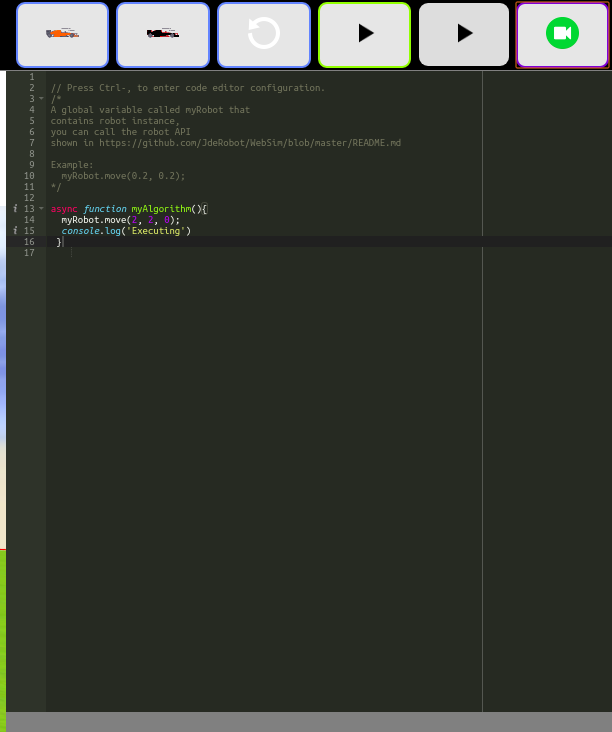
\includegraphics[scale=0.30]{img/competitiveEditorJavascript.png}
        \caption{Editor de \textit{JavaScript} para ejercicios competitivos}
        \label{fig:javascript_competitivo}
    \end{figure}
    
Cada uno de los botones tiene la funcionalidad de guardar el código escrito en el editor y, si se pulsa el botón del robot que no se está editando, se guarda el código y se carga el del otro robot en caso de que ya haya uno guardado. Si no hay ninguno se carga un editor vacío. 

\begin{lstlisting}[language=javascript]
var editFirst = true;
var editSecond = false;
var codeFirst = null;
var codeSecond = null;
  $('#firstRobot').click(()=>{
    if(editFirst){
      codeFirst = editor.getCode();
    }
    if(editSecond){
      codeSecond = editor.getCode();
      editSecond=false;
      if(codeFirst==null){
        editor.insertCode("",editor);
      }else{
        editor.insertCode(codeFirst,editor);
      }
    }
    editFirst= true;
  });
\end{lstlisting}

Cuando se pulsa el botón de ejecutar código, se ejecuta el método \textit{runBrain} del módulo \textit{brains} obteniendo previamente el código del robot que se esté editando.
\begin{lstlisting}[language=javascript]
  $("#runbtn").click(()=>{
     if (editFirst) {
       codeFirst = editor.getCode();
     } else {
       codeSecond = editor.getCode();
     }
    if (brains.threadExists(editorRobot1)){
      if (brains.isThreadRunning(editorRobot1)){
        brains.stopBrain(editorRobot1);
        brains.stopBrain(editorRobot2);
      }else{
        brains.resumeBrain(editorRobot1,codeFirst);
        brains.resumeBrain(editorRobot2,codeSecond);
      }
    }else{
      brains.runBrain(editorRobot1,codeFirst);
      brains.runBrain(editorRobot2,codeSecond);
    }
  });
\end{lstlisting}


La aplicación \textit{web} \textit{competitive-Scratch} se ha realizado de  manera similar, con la diferencia de que en este caso es necesario guardar el código de los bloques en \textit{XML} y su traducción en \textit{JavaScript}. Para realizarlo de forma limpia se ha creado un objeto que contiene un \textit{boolean} y dos cadenas de texto (\textit{listing} \ref{lst:savecode}). En el primero indica el código de qué \textit{robot} se está editando, en una cadena de texto se guarda el código \textit{XML} y en la otra su traducción en \textit{JavaScript}. Se puede ver la interfaz de este editor en la figura \ref{fig:scratch_competitivo}.
    \begin{figure}[H]
        \centering            
        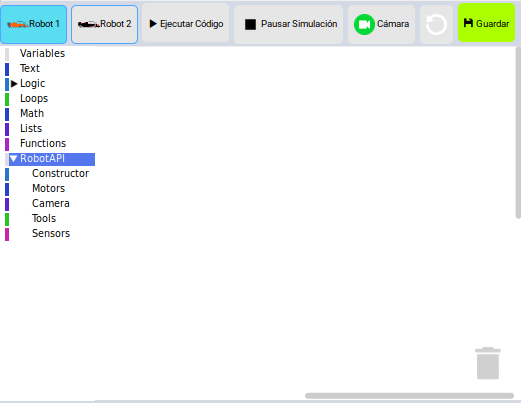
\includegraphics[scale=0.8]{img/competitivoEditorScratch.png}
        \caption{Editor de \textit{Scratch} para ejercicios competitivos}
        \label{fig:scratch_competitivo}
    \end{figure}

\begin{lstlisting}[language=javascript,label=lst:savecode, caption=código \textit{JavaScript} para guardar código de un robot]
var codeFirst = {
  js:"",
  xml:null,
  edit:true
};
var codeSecond = {
  js:"",
  xml: null,
  edit: false
};
  $('#firstRobot').click(()=>{
    if(codeFirst.edit){
      codeFirst.xml = editor.storeCode(editor.ui);
      editor.ui = editor.injectCode(editor.ui, codeFirst.xml);
    }
    if(codeSecond.edit){
      codeSecond.xml = editor.storeCode(editor.ui);
      codeSecond.edit = false;
      if(codeFirst.xml == null){
        editor.ui = editor.injectCode(editor.ui, '<xml></xml>');
      } else{
        editor.ui = editor.injectCode(editor.ui, codeFirst.xml);
      }
    }
    codeFirst.edit = true;
\end{lstlisting}

\begin{lstlisting}[language=javascript,caption=código \textit{JavaScript} para ejecutar código de los robots y guardar el que se está editando]
$("#runbtn").click(()=>{
    if (codeFirst.edit) {
        codeFirst.xml = editor.storeCode(editor.ui);
        editor.ui = editor.injectCode(editor.ui,codeSecond.xml);
        codeSecond.js = editor.getCode();
        editor.ui = editor.injectCode(editor.ui,codeFirst.xml);
        codeFirst.js = editor.getCode();
    } else {
        codeSecond.xml = editor.storeCode(editor.ui);
        editor.ui = editor.injectCode(editor.ui,codeFirst.xml);
        codeFirst.js = editor.getCode();
        editor.ui = editor.injectCode(editor.ui,codeSecond.xml);
        codeSecond.js = editor.getCode();
    }
    if (brains.threadExists(editorRobot1)){
      if (brains.isThreadRunning(editorRobot1)){
        brains.stopBrain(editorRobot1);
        brains.stopBrain(editorRobot2);
      }else{
        brains.resumeBrain(editorRobot1,codeFirst.js);
        brains.resumeBrain(editorRobot2,codeSecond.js);
      }
    }else{
      brains.runBrain(editorRobot1,codeFirst.js);
      brains.runBrain(editorRobot2,codeSecond.js);
    }
  });
\end{lstlisting}

Para puntuar el comportamiento de los robots de manera justa se han incluido en estos ejercicios \textit{evaluadores automáticos}. Van a tener diferentes comportamientos en cada ejercicio, por lo que se han desarrollado de tal forma que se pueda cargar cargar un evaluador distinto para cada uno o, incluso, no cargar ninguno. \newline

Para su implementación se ha creado el módulo \textit{evaluators}, que es similar a \textit{brains}. Tiene un método \textit{runEvaluator}, que acepta como parámetro un \textit{array} con los identificadores de los \textit{robots} a los que el código del evaluador debe conectarse para poder medir la calidad y el archivo del evaluador deseado. Este fichero se recoge como variable en el \textit{index.html} (listing \ref{lst:confEvaluator}) del editor correspondiente de forma similar a los archivos de configuración:
\begin{lstlisting}[language=html,label=lst:confEvaluator]
   <script>var config_evaluator = "evaluator_follow_line.js";</script> 
\end{lstlisting}

Para llamar a \textit{runEvaluator} se comprueba que se haya pasado un fichero en el \textit{index.html} en el código que inicializa el editor correspondiente: 

\begin{lstlisting}[language=html,label=lst:checkFile]
   if(typeof config_evaluator!=="undefined"){
    evaluators.runEvaluator([editorRobot1,editorRobot2],config_evaluator);
  }
\end{lstlisting}

En el método \textit{runEvaluator} se realiza un \textit{require} (que es la forma de importar módulos en \textit{JavaScript} de manera dinámica) de ese fichero, se crea la interfaz gráfica en el método \textit{evaluator.createInterface()} y se crea un objeto en el array de \textit{brains} que se ejecuta cada 400 milisegundos por medio del método \textit{evaluators.createTimeoutEvaluator}, que se apoya en la función \textit{setTimeout} de JavaScript. 


\begin{lstlisting}[language=javascript,caption={Funciones que crean el objeto para ejecutar el evaluador periódicamente}]
evaluators.runEvaluator = (arrayRobots,config_file)=>{
   evaluator = require("../assets/evaluators/"+config_file);
   evaluator.createInterface();
   brains.threadsBrains.push({
     "id": "evaluator",
     "running": true,
     "iteration": evaluators.createTimeoutEvaluator(arrayRobots,"evaluator"),
     "codeRunning": ""
   });
}
evaluators.createTimeoutEvaluator = (arrayRobots,id)=>{
  stopTimeoutRequested = false;
  let brainIteration = setTimeout(async function iteration(){
    evaluator.setEvaluator(arrayRobots);
    if (!stopTimeoutRequested) {
        var t = setTimeout(iteration, 400);
        var threadBrain = brains.threadsBrains.find((threadBrain)=> threadBrain.id == id);
        threadBrain.iteration = t;
    }
  }, 400);
  return brainIteration;
}
\end{lstlisting}


\subsection{Atraviesa-bosque competitivo}
\label{subsec:bosquecmp}
Este ejercicio es similar al escenario con un solo robot, pero en este caso se han creado dos pasillos en lugar de uno\footnote{\url{https://www.youtube.com/watch?v=v_aMvNPtncg}}. Se han añadido distintos objetos y elementos de \textit{A-Frame} en la misma ubicación para los dos \textit{robots} para que el recorrido sea justo.

Para su evaluador se crea una barra de progreso para cada robot y un cronómetro. Cuando se empiezan a mover los robots la barra de progreso empieza a completarse y el cronómetro se inicia, para comprobar el porcentaje completado se obtiene la posición del robot y la compara con el punto de llegada.

\begin{figure}[H]
\centering           
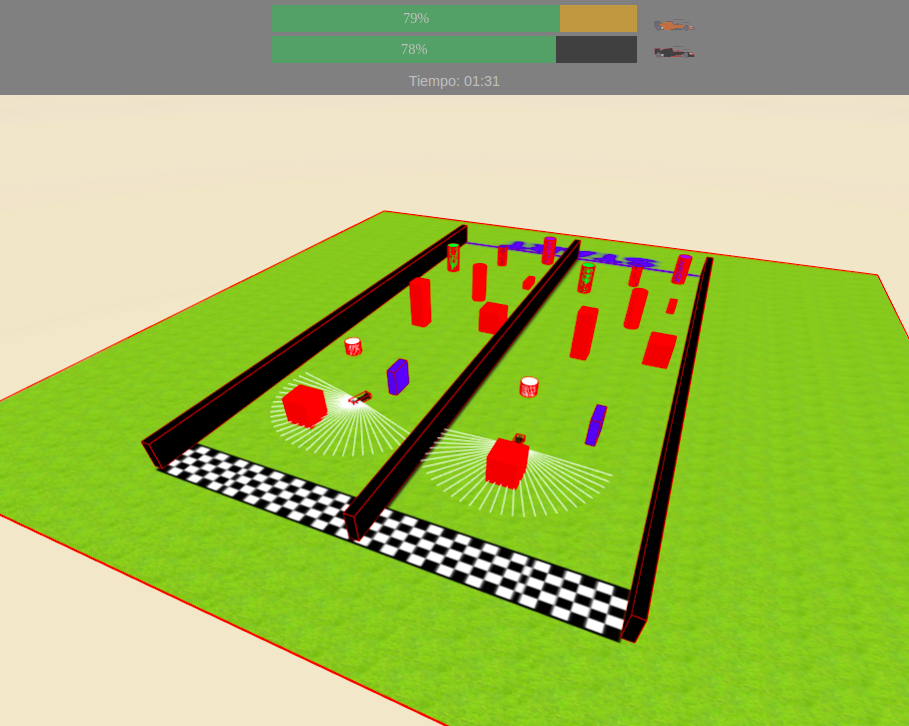
\includegraphics[scale=0.3]{img/evaluador_forest.png}
\caption{Escenario y evaluador para el ejercicio atraviesa-bosque}
\label{fig:evaluador_bosque}
\end{figure}


Las funciones necesarias para el evaluador se definen a continuación: 
\begin{itemize}
    \item Una dedicada a crear la interfaz que establece los elementos necesarios para añadir las barras de progreso, iconos, tiempo y sus atributos.
\begin{lstlisting}[language=javascript]
evaluator.createInterface= ()=>{
  var node = document.createElement("div");
  node.setAttribute("class","evaluator");
  var img1 = document.createElement("img");
  img1.setAttribute("class","carMarker");
  img1.setAttribute("src","../assets/resources/car1.svg")
  node.appendChild(img1);
  var node2 = document.createElement("div");
  node2.setAttribute("id","car1Progress");
  var node3 = document.createElement("div");
  node3.setAttribute("id","a-car1bar");
  node3.innerHTML = "0%";
  node2.appendChild(node3);
  node.appendChild(node2);
  var img2 = document.createElement("img");
  img2.setAttribute("class","carMarker");
  img2.setAttribute("src","../assets/resources/car2.svg")
  node.appendChild(img2);
  var node4 = document.createElement("div");
  node4.setAttribute("id","car2Progress");
  var node5 = document.createElement("div");
  node5.setAttribute("id","a-car2bar");
  node5.innerHTML = "0%";
  node4.appendChild(node5);
  node.appendChild(node4);
  var time = document.createElement("div");
  time.setAttribute("id","time");
  time.innerHTML="Tiempo: 00:00";
  time.style.marginTop="-87px";
  time.style.color="white";
  node.appendChild(time);
  var myiframe= document.getElementById("myIFrame");
  myiframe.insertBefore(node,myiframe.childNodes[0]);
}
\end{lstlisting}
    \item La función que se ejecuta periódicamente comprueba la velocidad de los robots y, si es mayor que 0, se inician los evaluadores, llama a una función que realiza la lógica para actualizar las barras de progreso y añadir un cronómetro al \textit{DOM}. La variable \textit{timeInit} se actualiza constantemente hasta que el usuario ejecuta su código y el \textit{robot} comienza a moverse, que se calcula el tiempo transcurrido y lo muestra en pantalla.
\begin{lstlisting}[language=javascript]
evaluator.setEvaluator = (arrayRobots) =>{
  let robot=Websim.robots.getHalAPI(arrayRobots[0]);
  if(!clock){
    timeInit = new Date();
  }
  if(robot.velocity.x>0){
    clock=true;
    var time= document.getElementById("time");
    progressBar(arrayRobots);
    var realTime = new Date(new Date() - timeInit);
    var formatTime = timeFormatter(realTime);
    time.innerHTML = "Tiempo: " + formatTime;
  }
}
\end{lstlisting}
    \item Función que calcula el porcentaje recorrido por cada uno de los \textit{robots}, modifica las barras de progreso y lo añade al \textit{DOM} para que aparezca en texto.
    
  \begin{lstlisting}[language=javascript]
function progressBar(arrayRobots){
  arrayRobots.forEach(function(robotID){
    let robot = Websim.robots.getHalAPI(robotID);
    var left=38.24 + robot.getPosition().x;
    var completed=(left*100)/78.48;
    var element = document.getElementById(robot.myRobotID+"bar");
    if((100-completed)>100){
      element.style.width = 100 + '%';
      element.innerHTML = 100 + '%';
    }else{
      element.style.width = Math.round(100-completed) + '%';
      element.innerHTML = Math.round(100-completed) + '%';
    }
  });
}
\end{lstlisting}
        \item Función que da formato al cronómetro.
\begin{lstlisting}[language=javascript]
function timeFormatter(time){
  var formatTime;
  if (time.getMinutes()<10){
    formatTime="0"+time.getMinutes();
  }else{
    formatTime=time.getMinutes();
  }
  formatTime+=":";
  if (time.getSeconds()<10){
    formatTime+="0"+time.getSeconds();
  }else{
    formatTime+=time.getSeconds();
  }
  return formatTime;
}
\end{lstlisting}
\end{itemize}

\subsection{Sigue-líneas competitivo}
\label{subsec:race}

En este ejercicio hay dos robots en el que tienen que seguir una linea de color blanco sobre fondo negro atravesando un puente en medio del circuito para que, de esta manera, ambos recorran la misma distancia\footnote{\url{https://www.youtube.com/watch?v=OaA7_wsXhk8}}.

La principal novedad del escenario es el puente creado, que permite ser cruzado mientras siguen la línea. La solución definitiva ha sido creando primitivas de \textit{A-Frame} (\textit{a-plane}) y añadiendo una textura diseñada con \textit{Photoshop} con el mismo aspecto que el resto del circuito.

El evaluador de este ejercicio es similar al de atraviesa-bosque, con la diferencia de que es necesario guardar en todo momento la posición y distancia recorrida por cada robot para calcular el porcentaje del circuito completado. 
\begin{lstlisting}[language=javascript,caption=Objeto creado para guardar posición y distancia recorrida de un robot]
var car={
    pos:{
        x:robot.getPosition().x,
        z:robot.getPosition().z
    },
    dist: 0
}
\end{lstlisting}

 \begin{lstlisting}[language=javascript,caption=Función que realiza la funcionalidad para rellenar la barra de progreso]
evaluator.setEvaluator = (arrayRobots) => {
  let robot1=Websim.robots.getHalAPI(arrayRobots[0]);
  let robot2=Websim.robots.getHalAPI(arrayRobots[1]);
  if(!clock){
    timeInit = new Date();
    car1 = {
        pos:{
                x:robot1.getPosition().x,
                z:robot1.getPosition().z
            },
            dist: 0
    };
    car2 = {
        pos:{
            x:robot2.getPosition().x,
            z:robot2.getPosition().z
        },
        dist: 0
    }
  }
  if(robot1.velocity.x>0){
    clock=true;
    var time= document.getElementById("time");
    progressBar(arrayRobots,[car1,car2]);
    var realTime = new Date(new Date() - timeInit);
    var formatTime = timeFormatter(realTime);
    time.innerHTML = "Tiempo: " + formatTime;
  }
}
\end{lstlisting}
            
\begin{figure}[H]
    \centering           
    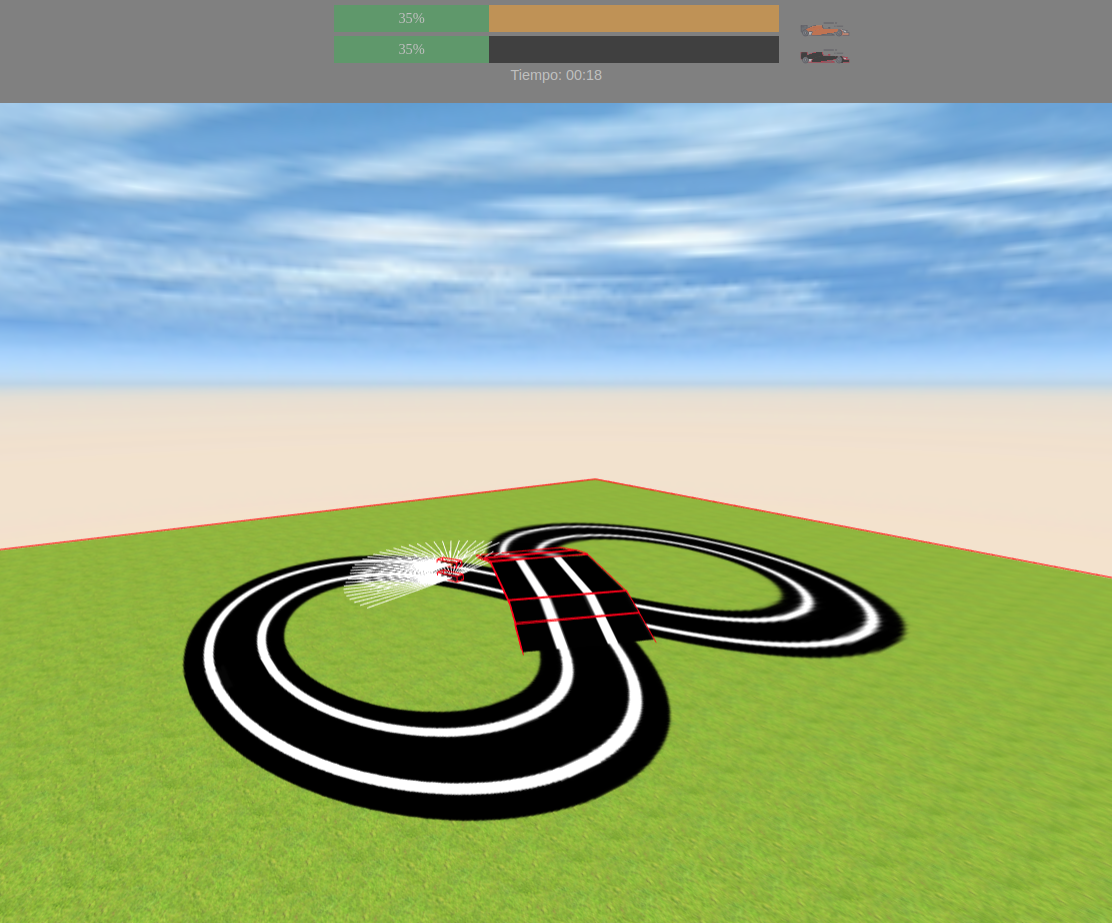
\includegraphics[scale=0.2]{img/evaluator_follow_line.png}
    \caption{Ejercicio y evaluador sigue-líneas competitivo}
    \label{fig:evaluador_siguelineas}
\end{figure}

\subsection{Gato-ratón}
\label{subsec:gatoraton}
No es estrictamente hablando un ejercicio competitivo directamente, con dos códigos de estudiantes sobre sendos robots en el mismo escenario simultáneamente. En este ejercicio hay dos robots, uno (el \textit{drone} gato) programado por el estudiante que hace el ejercicio y otro (el \textit{drone} ratón) programado por desarrolladores de la plataforma. 
En este ejercicio el usuario tiene que desarrollar su solución para que el \textit{robot} no se aleje del objetivo, el \textit{drone} ratón, que está en constante movimiento\footnote{\url{https://www.youtube.com/watch?v=xA9Emhdk_HQ}}. 

\begin{figure}[ht]
\centering           
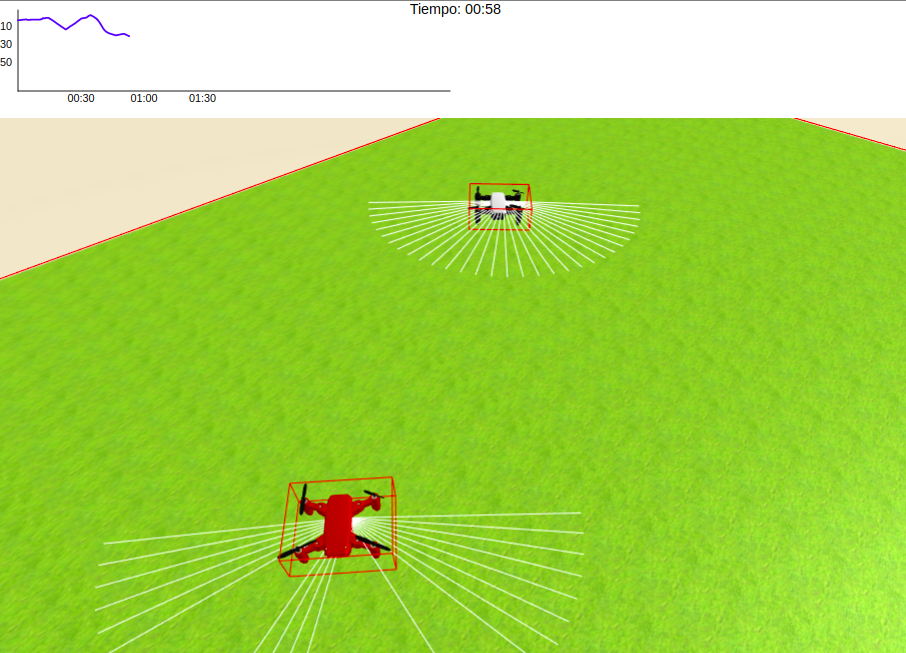
\includegraphics[scale=0.3]{img/evaluador_drone.png}
\caption{Evaluador y escenario con dos robots para ejercicio gato-ratón}
\label{fig:evaluador_gato_raton}
\end{figure}


Para este ejercicio se ha creado un \textit{script} llamado \textit{agents-methods.js}, basado en \textit{brains}, para ejecutar el código del \textit{drone} ratón sin necesidad de escribir código. Es muy similar al método \textit{runBrain} con la diferencia de que el código viene de un fichero en lugar del editor. En este módulo se guarda el código en la variable \textit{agents.code} con el siguiente código: 

\begin{lstlisting}[language=javascript]
agents.getCode = (file) => {
  var request = new XMLHttpRequest();
  request.open("GET", file);
  request.onreadystatechange = function () {
    if(request.status === 200 || request.status == 0) {
        agents.code = request.responseText;
    }
  }
  request.send();
}
\end{lstlisting}

Siendo \textit{file} una variable que se inicializa en el \textit{index.html} de manera similar a los ficheros de configuración y evaluadores automáticos. 
Una vez obtenido el código se llama al método \textit{runAgent} que recoge el código e incorpora la lógica programada en el \textit{array} de \textit{robots} del módulo \textit{brains}.

\begin{lstlisting}[language=javascript]
agents.runAgent = (robotID, code) =>{
  code = 'async function myAlgorithm(){\n'+code+'\n}\nmyAlgorithm();';
  brains.threadsBrains.push({
    "id": robotID,
    "running": true,
    "iteration": brains.createTimeoutBrain(code, Websim.robots.getHalAPI(robotID), robotID),
    "codeRunning": code
  });
}
\end{lstlisting}

A la hora de ejecutar el código, se elige si el código que se ejecuta es el que hay en el agente llamando al método \textit{runAgent} del módulo \textit{agents} o el que hay en el editor con el método \textit{runBrain} del módulo \textit{brains}. \\
En el siguiente código se ejecuta en un \textit{robot} el código escrito en el editor y en otro el escrito en el agente:

\begin{lstlisting}[language=javascript]
  $("#runbtn").click(()=>{
     if (editFirst) {
       codeFirst = editor.getCode();
     } else {
       codeSecond = editor.getCode();
     }
    if (brains.threadExists(editorRobot1)){
      if (brains.isThreadRunning(editorRobot1)){
        brains.stopBrain(editorRobot1);
        brains.stopBrain(editorRobot2);
      }else{
        brains.resumeBrain(editorRobot1,codeFirst);
        agents.resumeAgent(editorRobot2,agents.code);
      }
    }else{
      brains.runBrain(editorRobot1,codeFirst);
      agents.runAgent(editorRobot2,agents.code);
    }
  });\end{lstlisting}
  
  
Para el evaluador de este ejercicio se crea un gráfico con ayuda de una librería externa de \textit{JavaScript} (\textit{JavaScript Graphics Library}\cite{bib:jsgrafico}) que muestra la distancia entre \textit{drones} y el tiempo que lleva de ejecución. Se puede ver este evaluador en la figura \ref{fig:evaluador_gato_raton}. 
 En este caso, el método \textit{createInterface} realiza añade todo lo necesario al \textit{DOM} para que el gráfico sea completo y llama a la función \textit{setAxis()} para añadir los ejes y las etiquetas. \\
 
 \begin{lstlisting}[language=javascript,caption=Función que establece los ejes y etiquetas de la gráfica]
 evaluator.createInterface= ()=>{
  var node = document.createElement("div");
  node.setAttribute("id","panel");
  node.style.height="130px";
  node.style.backgroundColor="white";
  var time = document.createElement("div");
  time.setAttribute("id","time");
  time.marginLeft="50px";
  time.innerHTML="Tiempo: 00:00";
  time.style.color="black";
  time.style.textAlign="center";
  node.appendChild(time);
  var myiframe= document.getElementById("myIFrame");
  myiframe.insertBefore(node,myiframe.childNodes[0]);
  myPanel = new jsgl.Panel(document.getElementById("panel"));
  setAxis(myPanel);
  line = myPanel.createPolyline();
  line.getStroke().setColor('blue');
  line.getStroke().setWeight(2);
}
\end{lstlisting}

\begin{lstlisting}[language=javascript,caption=Método \textit{createInterface}]
function setAxis(myPanel){
  var axisX = myPanel.createLine();
  axisX.setStartPointXY(20,10);
  axisX.setEndPointXY(20,100);
  myPanel.addElement(axisX);
  var axisY = myPanel.createLine();
  axisY.setStartPointXY(20,100);
  axisY.setEndPointXY(500,100);
  myPanel.addElement(axisY);
  var myLabel = myPanel.createLabel();
  myLabel.setLocation(new jsgl.Vector2D(75,100));
  myLabel.setText("00:30");
  myPanel.addElement(myLabel);
  var myLabel = myPanel.createLabel();
  myLabel.setLocation(new jsgl.Vector2D(0,20));
  myLabel.setText("10");
  myPanel.addElement(myLabel);
}
\end{lstlisting}

\begin{lstlisting}[language=javascript,caption={Código JavaScript que calcula la distancia entre \textit{drones}, la representa e incorpora un cronómetro al \textit{DOM}}]
evaluator.setEvaluator = (arrayRobots) => {
  var robot1 = Websim.robots.getHalAPI(arrayRobots[0]);
  var robot2 = Websim.robots.getHalAPI(arrayRobots[1]);
  if(!clock){
    timeInit = new Date();
  }
  if(robot1.velocity.x >0 || robot2.velocity.x>0){
    clock = true;
    var time= document.getElementById("time");
    var realTime = new Date(new Date() - timeInit);
    var formatTime = timeFormatter(realTime);
    time.innerHTML = "Tiempo: " + formatTime;
    var pos1 = robot1.getPosition();
    var pos2 = robot2.getPosition();
    var dist = Math.sqrt(Math.pow(pos2.x-pos1.x,2)+
                         Math.pow(pos2.y-pos1.y,2)+
                         Math.pow(pos2.z-pos1.z,2));
    line.addPointXY(x,dist+10);
    x=x+0.5;
    myPanel.addElement(line);
  }
}
\end{lstlisting}
